\graphicspath{{Kapitel/Kapitel1_Einleitung/Images/}}

Der Einsatz künstlicher Intelligenzen ist aktuell in allen Bereichen der Informatik auf dem Vormarsch. Dies gilt vor allem für die Automobilindustrie, da das Thema des autonomen Fahrens nicht ohne intelligente Algorithmen realisierbar ist. Eine wichtige Rolle bei der Entwicklung solcher Algorithmen spielt dabei das maschinelle Lernen. Dabei wird versucht, ausgehend von vielen lehrreichen Beispieldaten, die Lösung einer Aufgabe zu lernen und auf andere unbekannte Daten zu verallgemeinern. So kann ein System auch auf vorher ungesehene Daten reagieren, was mit einer statischen Programmierung nur schwer oder gar nicht möglich ist. Der Erfolg dieses Prinzips hängt dabei stark von der Qualität der Beispieldaten ab von denen die Algorithmen lernen. Deshalb wird in die Erstellung dieser Daten sehr viel Arbeit gesteckt.\\

Im Bereich der Fahrerassistenzsysteme und des autonomen Fahrens ist es wichtig, dass das Auto seine Umgebung so gut wie möglich wahrnehmen kann. Algorithmen die für die Erkennung und Identifizierung des Umfeldes verantwortlich sind werden mit Daten von verschiedenen Sensoren gefüttert. Hierbei handelt es sich meist um Kamera-, Radar- oder LiDAR-Sensoren. Die Eingangsdaten dieser Sensoren müssen nun so aufbereiten werden, damit ein lernendes Computersystem etwas damit anfangen kann. Dazu werden alle, für das Anwendungsfeld wichtigen Teile mit entsprechenden Klassifikationen versehen. Diese Klassifikationen werden auch als \textit{Labels} oder \textit{Annotationen} bezeichnet. Zum Beispiel werden auf einem Kamerabild alle Personen und Fahrzeuge als eben diese markiert. Das Fahrzeug kann auf diese Weise lernen wie Personen und Fahrzeuge aussehen, um sie dann später im Straßenverkehr selbstständig wiederzuerkennen. Radar- und LiDAR-Sensoren liefern stattdessen Punktwolken als Eingangsdaten (vgl. Abbildung \ref{fig:Punktwolke}), das Prinzip bleibt allerdings das gleiche. Auch hier müssen alle wichtigen Teile, in diesem Fall Punkte, mit entsprechenden Klassen versehen werden. Dieser Vorgang nennt sich \textit{Labeln} bzw. \textit{Annotieren}.\\

\begin{figure}%
\centering
    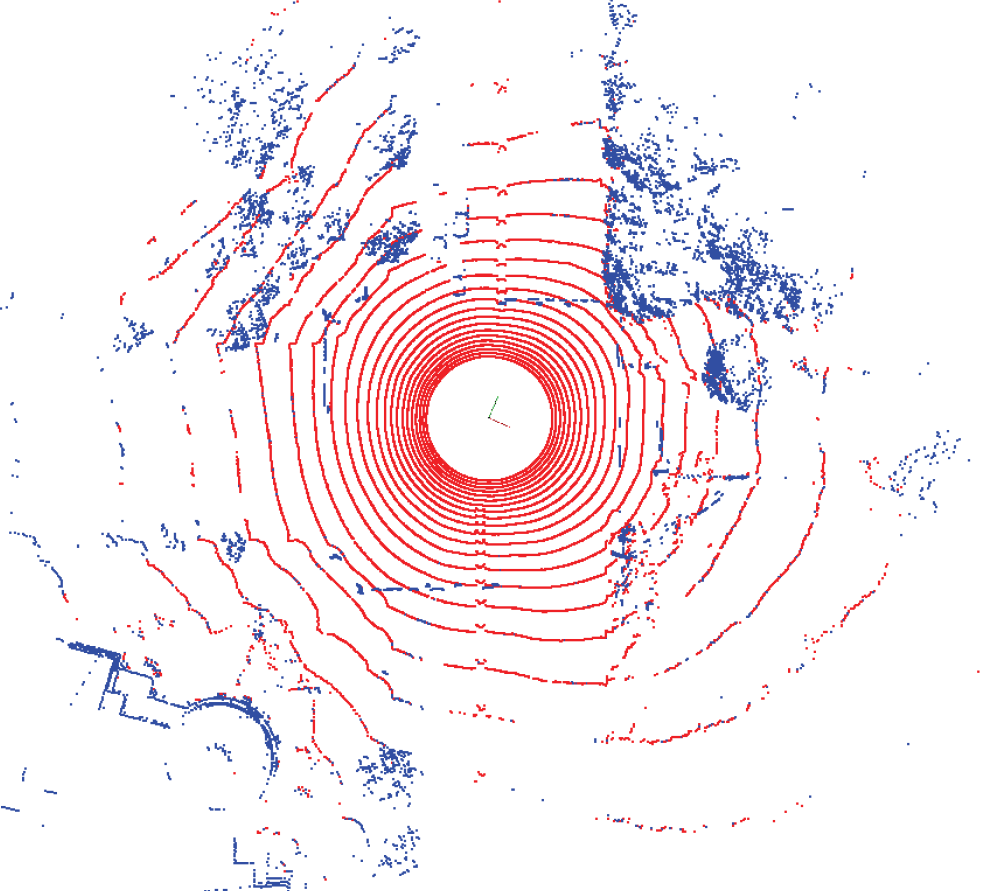
\includegraphics[width=7.5cm]{Punktwolke}
    \caption{Vogelperspektive auf eine LiDAR-Punktwolke, wobei die roten Punkte alle Boden- und die blauen alle Nicht-Bodenpunkte darstellen}
	\label{fig:Punktwolke}
\end{figure}

\section{Motivation}
Der Fokus dieser Arbeit liegt auf der Annotiation von Punktwolken. In einem bislang aufwändigen Verfahren (siehe Kapitel \ref{sec:C.LABEL}) müssen diese Punktwolken so aufbereitet und mit einer Bedeutung versehen werden, dass die Algorithmen an diesen Beispielen etwas lernen können. Sie müssen nach dem Lernen in der Lage sein Unterscheidungen und Erkennungen selbst durchzuführen und dabei möglichst wenige Fehler machen. Bei solchen Verfahren kommen Softwareanwendungen wie \textit{C.LABEL} zum Einsatz. Dies ist eine Anwendung zum Annotieren verschiedener Sensordaten für den Automobilbereich und wurde von der Firma \textit{CMORE Automotive GmbH} entwickelt. CMORE ist das betreuende Unternehmen dieser Masterarbeit und wird in Kapitel \ref{sec:CMORE} vorgestellt. Auf das Programm C.LABEL wird in Kapitel \ref{sec:C.LABEL} etwas genauer eingegangen. C.LABEL ist eine Anwendung, die zunächst die Sensordaten für den menschlichen Benutzer visualisiert. Dieser muss sie dann manuell mit unterschiedlichen Bedeutungen versehen. Wegen der großen Menge an Daten, die für das Trainieren der Algorithmen benötigt wird, muss dieses manuelle Annotieren möglichst effizient durchführbar sein.\\

Ein zweidimensionales Kamerabild kann sehr einfach auf einem Computermonitor dargestellt und bearbeitet werden. Eine besondere Herausforderung stellt jedoch die Verarbeitung von 3D-Daten, wie einer Punktwolke, dar. Hier stößt man mit den Möglichkeiten eines zweidimensionalen Computermonitors schnell an die Grenzen einer effizienten Darstellung und Bearbeitung. So ist es beispielsweise für die Annotierung solcher Punktwolken und ihrer Einzelmesswerte schwierig, die optimale Perspektive auf die Daten zu finden, die eine effiziente Erfassung durch den Menschen und eine entsprechende Bearbeitung zulässt. Dies erfordert von den Benutzern sehr viel Übung und Erfahrung, durch entsprechende Drehungen der Punktwolkendarstellung sich in dieser zurechtzufinden und Messpunkte realen Objekten zuzuordnen.\\ 

Eine Alternative dazu soll die Applikation bieten, die innerhalb dieser Masterarbeit entwickelt wurde. Diese soll das Visualisieren und Annotieren von Punktwolken einfacher und effizienter gestaltet. Mittels \textit{Virtual Reality (VR)} soll die Grenze zwischen 2-D und 3-D aufgehoben werden, sodass man sich als interaktiver Teilnehmer im dreidimensionalen Raum durch die Sensordaten navigieren, mit ihnen interagieren und sie annotieren kann. Die Applikation trägt den Namen \textit{C.LABEL-VR}.\\

\section{Ziel der Arbeit}
Ziel dieser Arbeit ist es zunächst ein passendes Medium für eine solche Applikation zu finden, das nicht nur die Anforderungen der Applikation selbst erfüllt, sondern auch an einem handelsüblichen Büro-Arbeitsplatz verwendet werden kann. Anschließend soll eine Applikation erstellt werden die folgende Grundfunktionalität erfüllt:\\

\begin{enumerate}
\item Mit der Anwendung soll es Möglich sein ein, bei CMORE gängiges, Datenformat einzulesen und alle nötigen Informationen daraus zu extrahieren

\item Aus den extrahierten Informationen soll eine Punktwolke generiert und innerhalb des gewählten Mediums visualisiert werden.

\item Der Benutzer muss die Möglichkeit haben durch die Punktwolke zu navigieren.

\item Die Applikation muss die Möglichkeit bieten jeden einzelnen Punkt mit einer Klassifikation versehen zu können. Dabei sollen Alleinstellungsmerkmale des gewählten Mediums benutzt werden, um eine vorzeigbare Verbesserung gegenüber der herkömmlichen Computer-Monitor-Annotation zu generieren. 

\item Alle getätigten Annotationen müssen in die eingelesenen Dateien zurückgeschrieben bzw. in neue Dateien exportiert werden.
\end{enumerate}

Anschließend sollen die Basisfunktionen erweitert und zusätzliche Funktionen hinzugefügt werden. Abhängig von der verbleibenden Zeit soll die Anwendung gemäß folgender Priorität erweitert werden:\\

\begin{enumerate}
\item Es sollen neue Möglichkeiten zur Annotation von Punkten implementiert werden.

\item Die Möglichkeit, eigene Klassifikationen für Punkte zu erstellen, soll hinzugefügt werden.

\item Neue Datenformate importieren.

\item Neue Navigationsmöglichkeiten implementieren.
\end{enumerate}

Am wichtigsten wäre hierbei also die Applikation um effiziente Möglichkeiten zum labeln von Punkten zu erweitern. Außerdem sollte es für den Benutzer möglich sein individuelle Klassifikationen anzulegen, um unterschiedliche Anwendungsgebiete abzudecken. Optional sind neue Navigationsmöglichkeiten und einlesbare Datenformate.

\section{Umfeld der Arbeit}
C.LABEL-VR und diese Masterarbeit wurden in Zusammenarbeit mit dem Unternehmen CMORE Automotive GmbH entwickelt. Als Grundlage für die Annotation von Punktwolken soll das CMORE-Programm C.LABEL dienen. Beides soll im Folgenden kurz vorgestellt werden. 

\subsection{CMORE Automotive GmbH}
\label{sec:CMORE}
Im Mai 2011 wurde die CMORE Automotive GmbH von Richard Woller und Gregor Matenaer die CMORE Automotive GmbH in Lindau gegründet. Der Tätigkeitsbereich von CMORE liegt in der Unterstützung Entwicklung und Validierung zukünftiger Mobilitätskonzepte. Dabei bietet CMORE Lösungen und Produkte für alle Entwicklungsphasen. Dazu gehören beispielsweise komplexe Steuergerätesoftware für die Serienproduktion, Deep Learning Verfahren und Softwaretools zur hochautomatisierten Datenanalyse oder auch komplette Fahrzeugmesstechniksysteme zur Referenzdatengenerierung. Seit 2017 gibt es innerhalb des Unternehmens eine eigene Abteilung, die verantwortlich für die Distribution, Analyse und Anreicherung von Daten im Automobilbereich ist. Sie trägt den Namen C.IDS (\textit{Integrated Data Solutions}). Ein Besipiel für solche Automobildaten sind Punktwolken von LiDAR-Sensoren, mit welchen sich auch diese Masterarbeit beschäftigt.     

\subsection{C.LABEL}
\label{sec:C.LABEL}
C.LABEL ist ein Programm zu Annotierung von Daten im zwei- und dreidimensionalen Bereich. Im zweidimensionalen Bereich handelt es sich bei den Daten um Kamerabilder. In diesen Bildern werden wichtige Objekte mit sogenannten \textit{Bounding Boxen} markiert, oder wichtige Bereiche werden zusammenhängend mit einer Klassifikation versehen (\textit{Semantisches Labeln}). Im dreidimensionalen Fall werden Punktwolken eines Radar- oder LiDAR-Sensors annotiert. Hierbei müssen alle wichtigen Punkte mit einer Klassifikation versehen werden. Die Labeling Methoden sind in Abbildung \ref{fig:LabelingMethoden} dargestellt. Das Ziel dieser Software ist es den Zeitaufwand, den die Annotation dieser Daten benötigt, zu minimieren. Dazu sind intelligente und effiziente Funktionen notwendig. Eine davon ist zum Beispiel die automatische Vorhersage von Annotationen durch stets analysierende Algorithmen. Dieses Prinzip wird \textit{Active Learning Loop} genannt. Bei der Entwicklung von C.LABEL-VR liegt der Fokus auf der Annotierung von 3D-Punktwolken und dabei wurden Funktionen und Ansätze von C.LABEL als Basis für die Entwicklung genutzt.

\begin{figure}%
    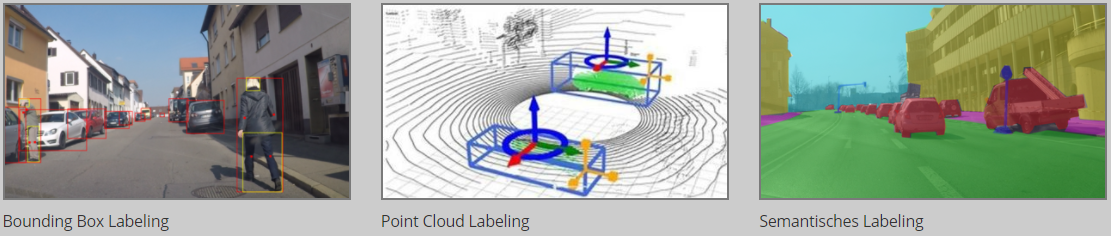
\includegraphics[width=14cm]{LabelingMethoden}
    \caption{Labeling Methoden in C.LABEL}
	\label{fig:LabelingMethoden}
\end{figure}